\chapter{Results}\label{chap:results}



In this section, we present the results of our study, which involved the generation of product descriptions for a sample of 100 randomly selected products from our dataset. Our goal was to systematically assess the impact of various factors on the quality and relevance of the generated descriptions. Following the methodology outlined in the previous chapter, we concentrated on variations in the prompt design, such as the incorporation of category descriptions and the number of shots used. We hope to determine which combinations produce the best results by carefully analyzing the outputs, allowing us to identify the most effective approaches for crafting accurate and engaging product descriptions.


Upon comparing the results across the six different prompt combinations, the evaluation based on Flesch Reading Ease reveals noteworthy insights. The boxplot(\autoref{fig:results_flesch}) analysis, showing the average scores for each combination, underscores that the zero-shot approach with the inclusion of category descriptions stands out as the most favorable option. This particular configuration achieves an average Flesch Reading Ease score of 30.87, Providing an appropriate level of readability for sufficient comprehension. These findings show the need of including category descriptions in a zero-shot context, highlighting the positive influence on output readability.

%\begin{figure}
%	\centering
%	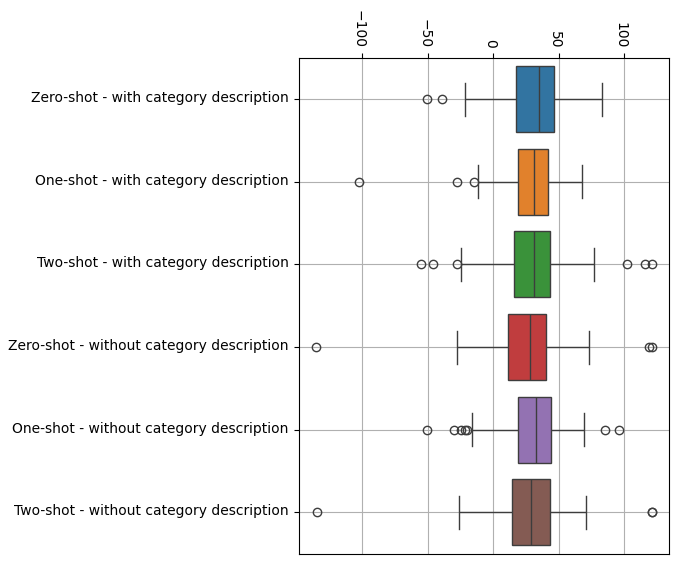
\includegraphics[width=1\linewidth]{result_flesch}
%	\caption{Flesch reading ease scores of outputs for the 100 randomly selected samples}
%	\label{fig:results_flesch}
%\end{figure}

\begin{figure}[H]
	\centering
	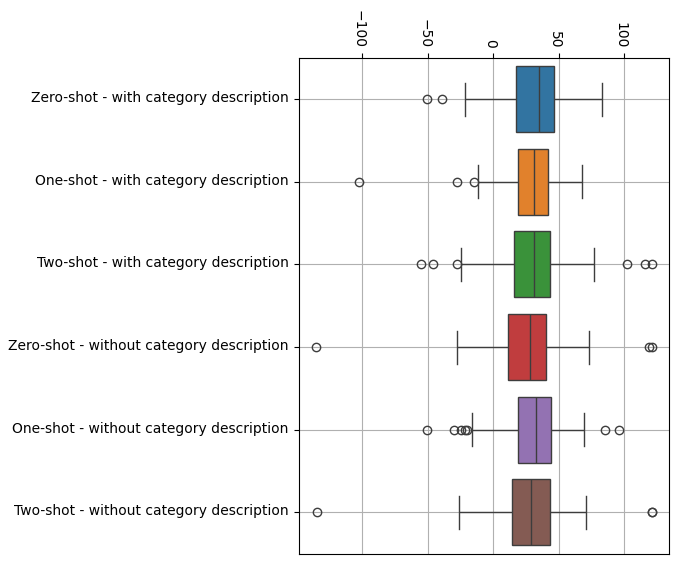
\includegraphics[width=0.8\linewidth]{result_flesch}
	\begin{tabular}{|l|l|l|l|l|}
		\hline
		\textbf{} & \textbf{mean} & \textbf{std} & \textbf{min} & \textbf{max} \\ \hline
		\textbf{\makecell{Zero-shot - \\ with category description}} & \textbf{30.87} & \textbf{25.22} & \textbf{-50.39} & \textbf{82.93} \\ \hline
		\textbf{\makecell{One-shot - \\ with category description}} & 28.00 & 22.69 & -102.80 & 68.04 \\ \hline
		\textbf{\makecell{Two-shot - \\ with category description}} & 30.50 & 26.67 & -55.60 & 121.22 \\ \hline
		\textbf{\makecell{Zero-shot - \\ without category description}} & 26.44 & 29.13 & -135.51 & 121.22 \\ \hline
		\textbf{\makecell{One-shot - \\ without category description}} & 29.85 & 23.42 & -51.02 & 95.84 \\ \hline
		\textbf{\makecell{Two-shot - \\ without category description} } & 26.64  & 29.19  & -134.61  & 121.22 \\ \hline
	\end{tabular}
	\captionlistentry[table]{Flesch reading ease scores of outputs for the 100 randomly selected samples}
	\captionsetup{labelformat=andtable}
	\caption{Flesch reading ease scores of outputs for the 100 randomly selected samples}
	\label{fig:results_flesch}
\end{figure}

\newpage
The class classification metric applied to the actual PBS descriptions for the sample dataset yields a 67\% accuracy. It's noteworthy that PBS claimed a +90\% accuracy, indicating that the randomly sampled dataset might present additional challenges compared to a typical scenario. This factor should be considered when interpreting the results of the class classification model.


In the evaluation of the six different prompt combinations using the class classification metric, our emphasis lies on the accuracy of classifications at level 3 and level 4, which represent a deeper and diverse categorizations. This is due to the fact that classifying Level 1 is straightforward, as almost 80\% of products fall under the category "Büromaterial, Büroeinrichtung, Bürotechnik, Papeterie". However, Levels 3 and 4 present challenges, with Level 4 being complex due to categories having fewer than 10 products in our dataset. In addition, since values are binary, the ground truth is consistently true, and the data is unbalanced, it may be better to evaluate the model by using accuracy, since it provides a straightforward measure of how well the instances classified.

Analyzing the accuracy across these levels, the plot (\autoref{fig:results_cc}) illustrates that the zero-shot options, both with and without category descriptions, exhibit comparable results. Specifically, the zero-shot with category description excels in achieving superior accuracy at level 3, while the zero-shot without category description shows an advantage in accuracy at level 2. Given our emphasis on the more challenging and intricate categorizations at levels 3 and 4, the zero-shot with category description appears as the more favorable option.


 

\begin{figure}[H]
	\centering
	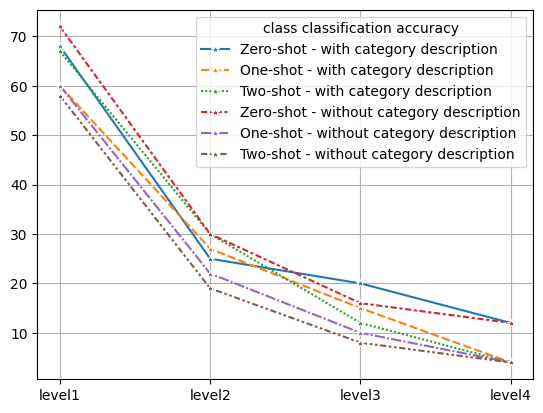
\includegraphics[width=1\linewidth]{result_cc}
	\caption{Class classification accuracy for each level of outputs for the 100 randomly selected samples}
	\label{fig:results_cc}
\end{figure}

It appears that there is minimal variation between different setups when it comes to complex word count levels. However, the approaches zero-shot with and without category description and also one-shot with category description show the lowest count of complex words (\autoref{fig:result_complex_word}). 

%\begin{figure}
%	\centering
%	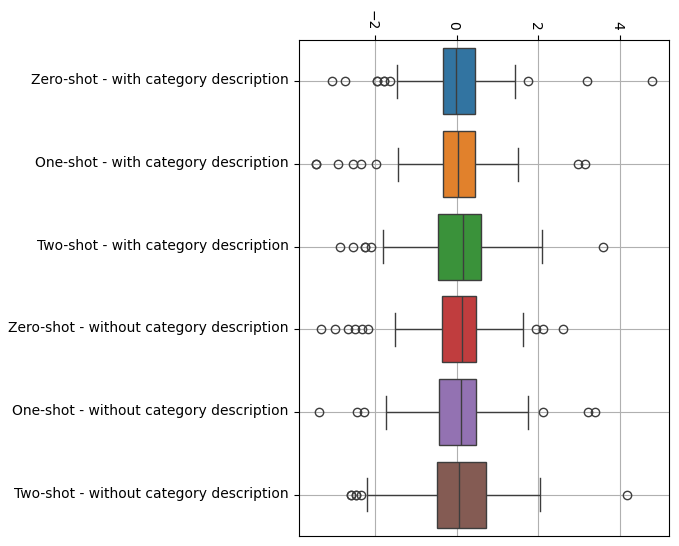
\includegraphics[width=1\linewidth]{result_complex_word}
%	\caption{normalized count of complex words of outputs for the 100 randomly selected samples}
%	\label{fig:result_complex_word}
%\end{figure}

\begin{figure}[H]
	\centering
	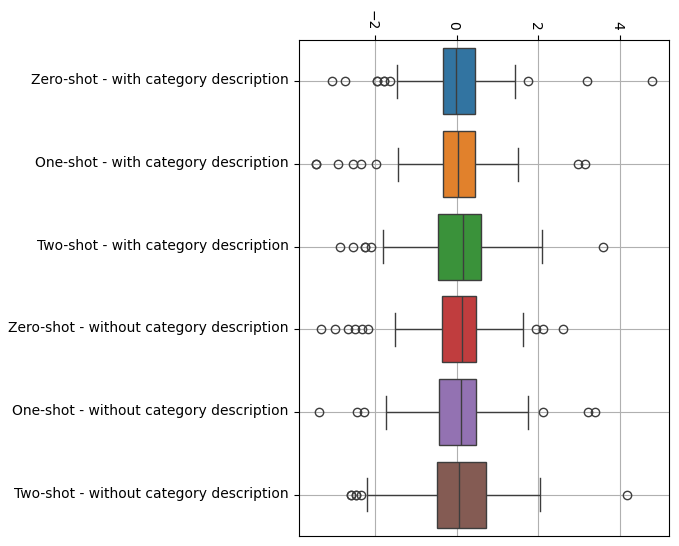
\includegraphics[width=0.8\linewidth]{result_complex_word}
	\begin{tabular}{|l|l|l|l|l|}
		\hline
		\textbf{} & \textbf{mean} & \textbf{std} & \textbf{min} & \textbf{max} \\ \hline
		\textbf{\makecell{Zero-shot - \\ with category \\ description}} & -9.32e-17 & 1.00e+00 & -3.06e+00 & 4.78e+00 \\ \hline
		\textbf{\makecell{One-shot - \\ with category \\ description}} & \textbf{-4.62e-18} & \textbf{1.00e+00} & \textbf{-3.44e+00} & \textbf{3.14e+00} \\ \hline
		\textbf{\makecell{Two-shot - \\ with category \\ description}}& 1.59e-16 & 1.00e+00 & -2.84e+00 & 3.59e+00 \\ \hline
		\textbf{\makecell{Zero-shot - \\ without category \\ description}} & -8.88e-17 & 1.00e+00 & -3.31e+00 & 2.60e+00 \\ \hline
		\textbf{\makecell{One-shot - \\ without category \\ description}} & -1.94e-16 & 1.00e+00 & -3.36e+00 & 3.39e+00 \\ \hline
		\textbf{\makecell{Two-shot - \\ without category \\ description} } & 1.61e-16  & 1.00e+00  & -2.59e+00  & 4.17e+00 \\ \hline
		
	\end{tabular}
	\captionlistentry[table]{Normalized count of complex words of outputs for the 100 randomly selected samples}
	\captionsetup{labelformat=andtable}
	\caption{Normalized count of complex words of outputs for the 100 randomly selected samples}
	\label{fig:result_complex_word}
\end{figure}

In summary, the zero-shot with category description stands out as the most effective option, demonstrating satisfactory accuracy, especially in challenging categorizations at levels 3 and 4. While not flawless, this approach strikes a reasonable balance between automation and accuracy in generating product descriptions.

\section{The effects of different components in our pipeline}

This section dives into the various components of our pipeline and how they affect our results. We investigate the effects of altering variables like temperature, using formal prompt styles, and incorporating post-processing techniques. By examining these various elements, we can uncover the influences that each component has on the overall performance of our system.


\subsection{Bloom vs other LLMs}\label{comparison-of-llms}


As part of our initial research, we compared text generation abilities of various German language models, specifically focusing on GPT-2,  GPT-2-Wechsel-German, Mistral and 
EM\_German\_mistral we employed a specific product description prompt to assess their performance. The prompt was crafted as follows:

{\tiny
	\begin{lstlisting}[breaklines=true, caption={prompt used for GPT-2 and GPT-2-Wechsel-German}, captionpos=b]
		
		Schreiben Sie eine Produktbeschreibung für das folgende Produkt: \n Produktname: Lasertoner cyan OKI 42804547 \n Produktkategorie: Toner, Tonereinheit (Laserdrucker, Kopierer)\n. Produktbeschreibung:
		
	\end{lstlisting}
}


The outcomes from GPT-2 (\autoref{gpt2}) exhibited notable limitations. The generated text (\autoref{gpt2-result}) lacked coherence and meaning, incorporating English phrases, a reflection of its primary training in English. This linguistic mismatch resulted in outputs that were incomprehensible and not aligned with the specified German product category. Furthermore, GPT-2's struggle to handle the German language was evident in its output, illustrating the significance of language-specific training for accurate text generation.

\begin{center}
	\fbox{\begin{varwidth}{\textwidth}
			
			\begin{flushleft}
				Produkt: Zug-Das-Dreiner, Die Geburtung, Lautenberg Produktkriegsprodut und dazsühle Kultura-Sonderstahl zu den Dägen (Sterzweil und Zuger), Lautenberg Produktkognizativ, Weltung Produkt.  (Druktur) The production number in the field of Kautenberg was changed for K-Kutur by the production department.The following is also available from: Lüztannen, d. 1945-01 The Production of D-Draken (The Kautenberg, 1933 - 1954. The Kulturer, 1939. K-Kützreiter, 1945) (Aktroniekt: Draken, Torskeller, Kauttern) - Läsgebung (K-Drapfach, 1933) (The Kautenberg, 1937 - 1938) - Zügekommen - Kautzenkultur. Zum zum Kütschendes, Kautzer (Draken: Drapfisch, Gekorung) and the Kulturers. Zuscheren (S-Drapfen). Lager-Lager. Lagerlager. Kängekultur und lautter Lachnachlung. Kautzenfach (Hochlager): Lauttern (Lauchmer). The production of a single Lager-Bauchter, the Larger, and the bigger a smaller are
			\end{flushleft}
	\end{varwidth}}\par
	\captionof{Example}{The product description generated using GPT-2\label{gpt2-result}}
	
\end{center}

Turning to GPT-2-Wechsel-German(\autoref{gpt2}), the generated content (\autoref{german-gpt2-result}) was characterized by repetitiveness and a lack of informative details. Notably, it tended to reproduce the input data rather than providing novel and relevant product descriptions. This behavior is indicative of a failure to grasp the intent of the prompt and generate contextually appropriate content.

\begin{center}
	\fbox{\begin{varwidth}{\textwidth}
			
			\begin{flushleft}
				Produktname: Toner, Tonerreinheit (Laserdrucker, Kopierer) - Toner, Tonerreinheit (Laserdrucker, Kopierer)Produktname: Toner, Tonerreinheit (Laserdrucker, Kopierer) - Toner, Tonerreinheit (Laserdrucker, Kopierer)Produktname: Toner, Tonerreinheit (Laserdrucker, Kopierer) - Toner, Tonerreinheit (Laserdrucker, Kopierer)Produktname: Toner, Tonerreinheit (Laserdrucker, Kopierer) - Toner, Tonerreinheit (Laserdrucker, Kopierer)Produktname: Toner, Tonerreinheit (Laserdrucker, Kopierer) - Toner, Tonerreinheit (Laserdrucker, Kopierer)Produktname: Toner, Tonerreinheit (Laserdrucker, Kopierer) - Toner, Tonerreinheit (Laserdrucker, Kopierer)Produktname: Toner, Tonerreinheit (Laserdrucker, Kopierer) - Toner, Tonerreinheit (Laserdrucker, Kopierer)Produktname: Toner, Tonerreinheit (Laserdrucker, Kopierer) - Toner, Tonerreinheit (Laserdrucker, Kopierer)Produktname: Toner, Tonerreinheit 
			\end{flushleft}
	\end{varwidth}}\par
	\captionof{Example}{The product description generated using GPT-2-Wechsel-German\label{german-gpt2-result}}
\end{center}


In comparing Mistral and Bloom for German text generation, we utilized the same prompt as GPT-2. However, Mistral's output resulted in a series of empty lines, providing no meaningful content (\autoref{mistral-result}).We received a response that contained several product features from em\_german\_mistral, fine-tuned version of Mistral on german language.
In spite of the output (\autoref{german-mistral-result}) demonstrating relevant details about the product, it contained inaccuracies, such as fabricated model numbers, and differed from our preferred structure. It is possible to partially solve these problems through prompt engineering, however.

\begin{center}
	\fbox{\begin{varwidth}{\textwidth}
			
			\begin{flushleft}
				\textbackslash n\textbackslash n\textbackslash n\textbackslash n\textbackslash n\textbackslash n\textbackslash n\textbackslash n\textbackslash n\textbackslash n\textbackslash n\textbackslash n\textbackslash n\textbackslash n\textbackslash n\textbackslash n\textbackslash n\textbackslash n\textbackslash n\textbackslash n\textbackslash n\textbackslash n\textbackslash n\textbackslash n\textbackslash n\textbackslash n\textbackslash n\textbackslash n\textbackslash n\textbackslash n\textbackslash n\textbackslash n\textbackslash n\textbackslash n\textbackslash n \textbackslash n\textbackslash n\textbackslash n\textbackslash n\textbackslash n\textbackslash n\textbackslash n\textbackslash n\textbackslash n\textbackslash n\textbackslash n\textbackslash n\textbackslash n\textbackslash n\textbackslash n\textbackslash n\textbackslash n\textbackslash n\textbackslash n\textbackslash n\textbackslash n\textbackslash n\textbackslash n\textbackslash n\textbackslash n\textbackslash n\textbackslash n\textbackslash n\textbackslash n\textbackslash n\textbackslash n\textbackslash n\textbackslash n\textbackslash n\textbackslash n \textbackslash n\textbackslash n\textbackslash n\textbackslash n\textbackslash n\textbackslash n\textbackslash n\textbackslash n\textbackslash n\textbackslash n\textbackslash n\textbackslash n\textbackslash n\textbackslash n\textbackslash n\textbackslash n\textbackslash n\textbackslash n\textbackslash n\textbackslash n\textbackslash n\textbackslash n\textbackslash n
			\end{flushleft}
	\end{varwidth}}\par
	\captionof{Example}{The product description generated using Mistral 7B\label{mistral-result}}
\end{center}


\begin{center}
	\fbox{\begin{varwidth}{\textwidth}
			\begin{flushleft}
				Produktmerkmale:
				
				* Cyan Toner für Laserdrucker und Kopierer \newline
				* Hergestellt von OKI \newline
				* Modellnummer: 42804547 \newline
				* Pass zu den folgenden Modellen: OKI C331, OKI C332, OKI C333, OKI C334, OKI C341, OKI C342, OKI C343, OKI C344, OKI C431, OKI C432, OKI C433, OKI C434, OKI C531, OKI
			\end{flushleft}
	\end{varwidth}}\par
	\captionof{Example}{The product description generated using em\_german\_mistral\label{german-mistral-result}}
	
\end{center}

Upon comparing the Bloom model outputs, a significant difference emerges between the English and German versions. The English Bloom model appears to generate less informative descriptions (\autoref{bloom-basic-result}) in german language, often repeating the product name and including a fake website link. In contrast, the German Bloom model generates more coherent and contextually relevant text (\autoref{german-bloom-basic-result}) that effectively describes the product. However, it is critical to recognize the presence of hallucinations in the German output, as shown by the inclusion of a made-up website link and phone number. 

\begin{center}
	\fbox{\begin{varwidth}{\textwidth}
			
			\begin{flushleft}
				Lasertoner cyan OKI 42804547 \textbackslash n
				Produktlink: http://www.example.com/
			\end{flushleft}
	\end{varwidth}}\par
	\captionof{Example}{The product description generated using Bloom\label{bloom-basic-result}}
\end{center}


\begin{center}
	\fbox{\begin{varwidth}{\textwidth}
			\begin{flushleft}
				Original-Tonerkartusche in schwarzer Farbe. Passend zum oben angegebenen Druckermodell.. Für die Druckqualität und -reichweite sind nur originalgetreue Produkte von Markenherstellern geeignet! Wir beraten auch gern zu dem Thema kompatible Artikel wie hier beschrieben per EMail oder Telefon 0431 / 66051290Sie befinden sich aktuell auf unserer Partnerseite https://www\u200btipicobetbrightonandhoveunitedukcom/de/. Loggen sie diese Seite über
			\end{flushleft}
	\end{varwidth}}\par
	\captionof{Example}{The product description generated using German Bloom\label{german-bloom-basic-result}}
	
\end{center}

In contrast, German Bloom model(\autoref{german-bloom}) demonstrated linguistic accuracy, coherence, and relevance in generating meaningful product descriptions. The results from the Bloom model aligned with the provided prompt, showcasing the model's proficiency in comprehending and accurately responding to German language prompts in the specified product category.



\subsection{Unspecified prompt style vs formal prompt style}\label{prompt-style}

The inclusion of prompt style, specifically "formal," in our prompt, introduced an interesting variable in our study. We maintained consistency in other aspects, following the best-case scenario of zero-shot with category description. The results, however, revealed a potential negative impact of prompt style. In the class classification metric, accuracy for levels 3 and 4 decreased, indicating that the introduction of a formal style might interfere with the model's ability to accurately classify more complex and diverse products(\autoref{fig:results_cc_prompt_style}). Additionally, the average Flesch reading ease score, a measure of text readability, showed a decrease, suggesting that the formal style might contribute to a less accessible and less comprehensible output(\autoref{fig:results_flesch_prompt_style}). These findings emphasize the importance of carefully considering the inclusion of prompt styles and their potential implications on the generated product descriptions.


%\begin{figure}[H]
%	\centering
%	\begin{minipage}{.5\textwidth}
%		\centering
%		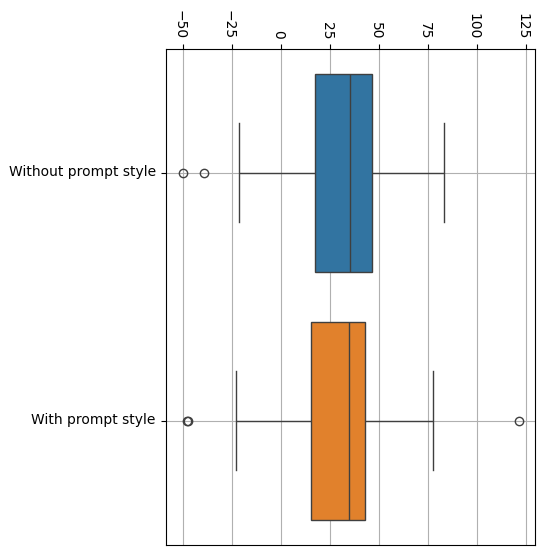
\includegraphics[width=1\linewidth]{results_flesch_prompt_style}
%		\caption{The impact of prompt style on Flesch reading ease score for the 100 randomly selected samples}
%		\label{fig:results_flesch_prompt_style}
%	\end{minipage}%
%	\begin{minipage}{.5\textwidth}
%		\centering
%		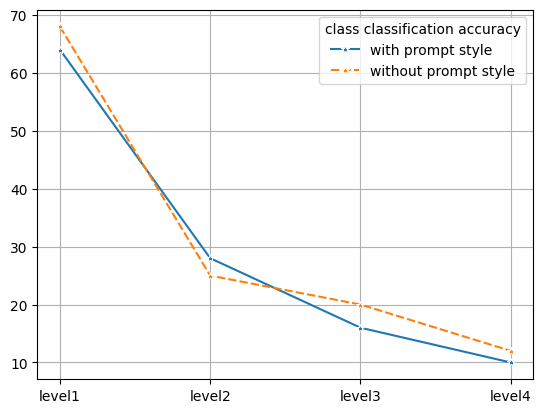
\includegraphics[width=1\linewidth]{results_cc_prompt_style}
%		\caption{The impact of prompt style on class classification accuracy for the 100 randomly selected samples}
%		\label{fig:results_cc_prompt_style}
%	\end{minipage}
%\end{figure}

\begin{figure}[H]
	\centering
	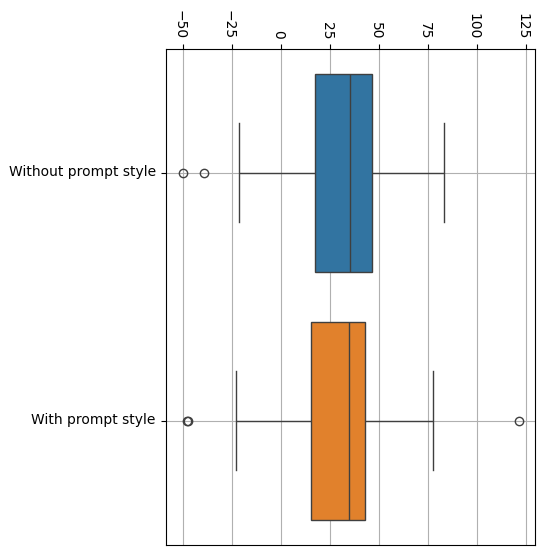
\includegraphics[width=0.5\linewidth]{results_flesch_prompt_style}
	\begin{tabular}{|l|l|l|l|l|}
		\hline
		\textbf{} & \textbf{mean} & \textbf{std} & \textbf{min} & \textbf{max} \\ \hline
		\textbf{Without prompt style} & \textbf{30.87} & \textbf{25.22} & \textbf{-50.39} & \textbf{82.93} \\ \hline
		\textbf{With prompt style } & 29.59  & 24.02  & -47.98  & 121.22 \\ \hline
	\end{tabular}
	\captionlistentry[table]{The impact of prompt style on Flesch reading ease score for the 100 randomly selected samples}
	\captionsetup{labelformat=andtable}
	\caption{The impact of prompt style on Flesch reading ease score for the 100 randomly selected samples}
	\label{fig:results_flesch_prompt_style}
\end{figure}

\begin{figure}[H]
	\centering
	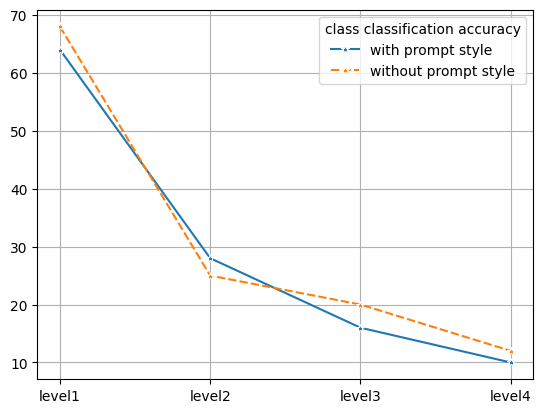
\includegraphics[width=0.8\linewidth]{results_cc_prompt_style}
	\caption{The impact of prompt style on class classification accuracy for the 100 randomly selected samples}
	\label{fig:results_cc_prompt_style}
\end{figure}

\subsection{Effect of post-processing}\label{post-processing}

In evaluating the influence of the post-processing step on the output, we conducted a comparison between descriptions before and after post-processing, With the focus on the zero shot setup with category descriptions. In alignment with our best-performing case, the study maintained consistency in all other parameters. The results indicate a complex impact of post-processing on different metrics.


%\begin{figure}[H]
%	\centering
%	\begin{minipage}{.5\textwidth}
%		\centering
%		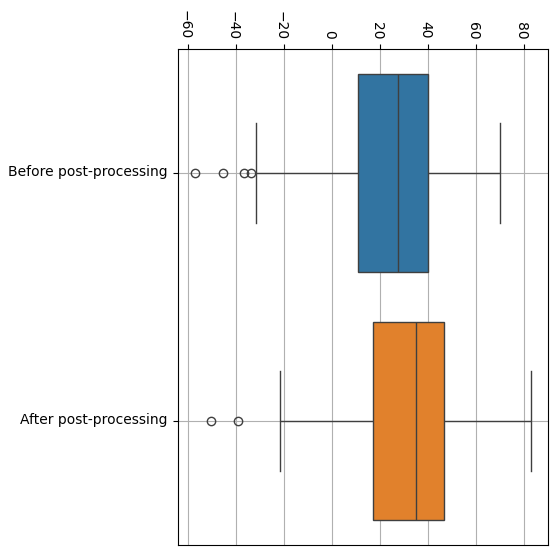
\includegraphics[width=1\linewidth]{result_flesch_postprocessing}
%		\caption{The impact of post-processing on Flesch reading ease score for the 100 randomly selected samples}
%		\label{fig:result_flesch_postprocessing}
%	\end{minipage}%
%	\begin{minipage}{.5\textwidth}
%		\centering
%		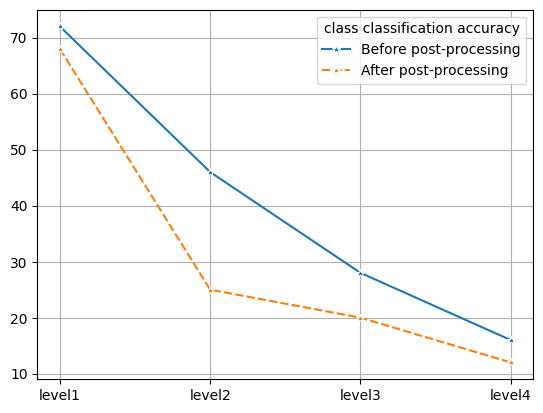
\includegraphics[width=1\linewidth]{result_cc_postprocessing}
%		\caption{The impact of post-processing on class classification accuracy for the 100 randomly selected samples}
%		\label{fig:result_cc_postprocessing}
%	\end{minipage}
%
%\end{figure}

\begin{figure}[H]
	\centering
	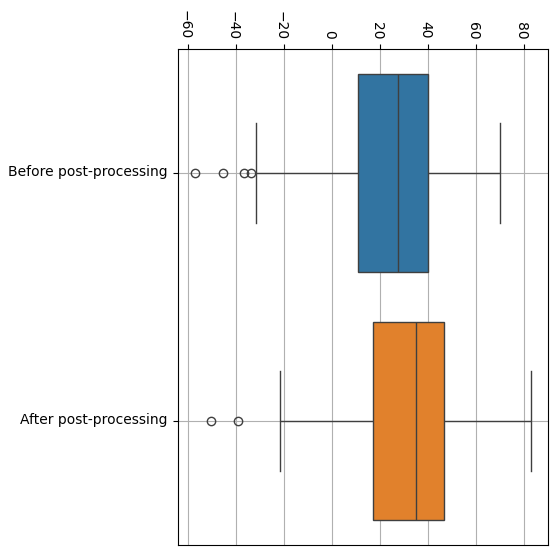
\includegraphics[width=0.5\linewidth]{result_flesch_postprocessing}
	\begin{tabular}{|l|l|l|l|l|}
		\hline
		\textbf{} & \textbf{mean} & \textbf{std} & \textbf{min} & \textbf{max} \\ \hline
		\textbf{Before post-processing} & 22.83 & 23.48 & -57.09 & 69.78 \\ \hline
		\textbf{After post-processing } & \textbf{30.87}  & \textbf{25.22}  & \textbf{-50.39}  & \textbf{82.93} \\ \hline
	\end{tabular}
	\captionlistentry[table]{The impact of post-processing on Flesch reading ease score for the 100 randomly selected samples}
	\captionsetup{labelformat=andtable}
	\caption{The impact of post-processing on Flesch reading ease score for the 100 randomly selected samples}
	\label{fig:result_flesch_postprocessing}
\end{figure}


\begin{figure}[H]
	\centering
	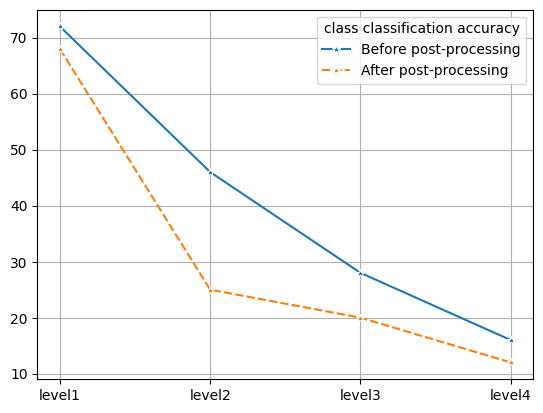
\includegraphics[width=0.8\linewidth]{result_cc_postprocessing}
	\caption{The impact of post-processing on class classification accuracy for the 100 randomly selected samples}
	\label{fig:result_cc_postprocessing}
\end{figure}

Class classification accuracy exhibited a notable decrease across all levels after post-processing (\autoref{fig:result_cc_postprocessing}). This suggests that while post-processing may enhance readability, it introduces changes that may compromise the model's ability to accurately classify products into specific categories, particularly for more complex categories.

However, the average Flesch reading ease score showed a substantial increase after post-processing (\autoref{fig:result_flesch_postprocessing}). This suggests that the post-processing step contributes positively to the overall readability of the generated product descriptions. Despite the trade-off in class classification accuracy, the improved Flesch reading ease score indicates a potential enhancement in the linguistic quality and accessibility of the final product descriptions. This trade-off highlights the delicate balance between preserving accuracy in classification and optimizing linguistic clarity in the post-processing phase.

\subsection{Using different subsets of features}\label{feature-subsets}

In our examination of how different feature subsets in the prompt affect the output, we used the optimal configuration of zero-shot with category description. We specifically tested the influence of including product brand and manufacturer information. In terms of class classification, the inclusion of brand and manufacturer details led to decreased accuracy, especially in intricate classifications (levels 3 and 4) (\autoref{fig:results_cc_feature}). The average Flesch reading ease score also slightly decreased (\autoref{fig:results_flesch_feature}), suggesting a trade-off between additional context and a potential reduction in precision and readability. Careful consideration of prompt elements is crucial for optimizing the model's performance in generating accurate and clear product descriptions.



%\begin{figure}[H]
%	\centering
%	\begin{minipage}{.5\textwidth}
%		\centering
%		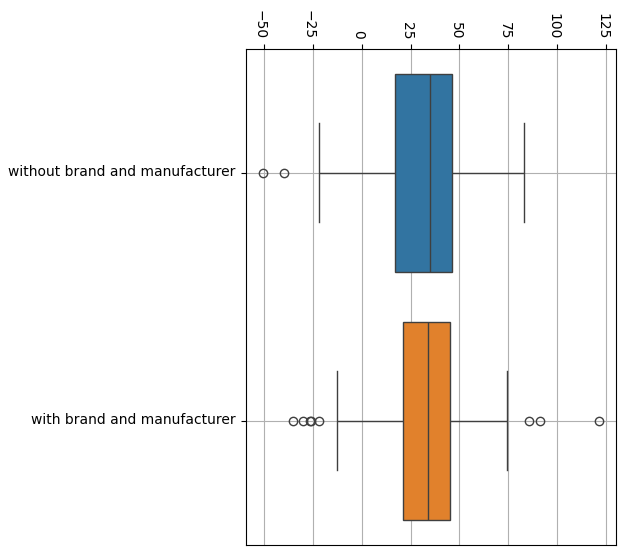
\includegraphics[width=1\linewidth]{results_flesch_feature}
%		\caption{The impact of inlcuding brand and manufacturer in the prompt on Flesch reading ease score for the 100 randomly selected samples}
%		\label{fig:results_flesch_feature}
%	\end{minipage}%
%	\begin{minipage}{.5\textwidth}
%		\centering
%		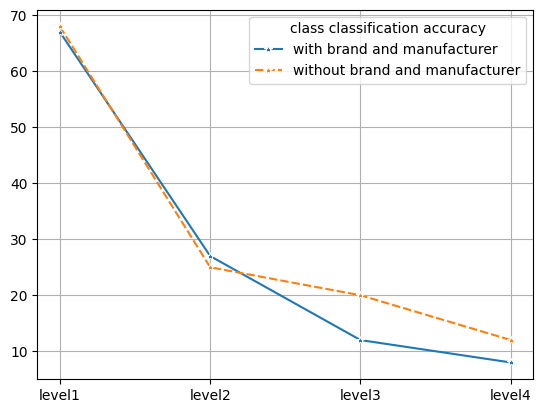
\includegraphics[width=1\linewidth]{results_cc_feature}
%		\caption{The impact of inlcuding brand and manufacturer in the prompt on class classification accuracy for the 100 randomly selected samples}
%		\label{fig:results_cc_feature}
%	\end{minipage}
%\end{figure}

\begin{figure}[H]
	\centering
	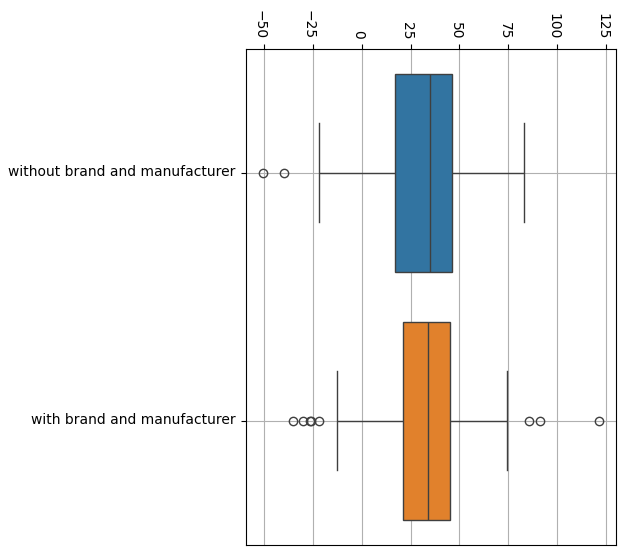
\includegraphics[width=0.5\linewidth]{results_flesch_feature}
	\begin{tabular}{|l|l|l|l|l|}
		\hline
		\textbf{} & \textbf{mean} & \textbf{std} & \textbf{min} & \textbf{max} \\ \hline
		\textbf{\makecell{without brand \\ and manufacturer}} & \textbf{30.87} & \textbf{25.22} & \textbf{-50.39} & \textbf{82.93} \\ \hline
		\textbf{\makecell{with brand \\and manufacturer }} & 29.93  & 24.92  & -35.11  & 121.22 \\ \hline
	\end{tabular}
	\captionlistentry[table]{The impact of inlcuding brand and manufacturer in the prompt on Flesch reading ease score for the 100 randomly selected samples}
	\captionsetup{labelformat=andtable}
	\caption{The impact of inlcuding brand and manufacturer in the prompt on Flesch reading ease score for the 100 randomly selected samples}
	\label{fig:results_flesch_feature}
\end{figure}

\begin{figure}[H]
	\centering
	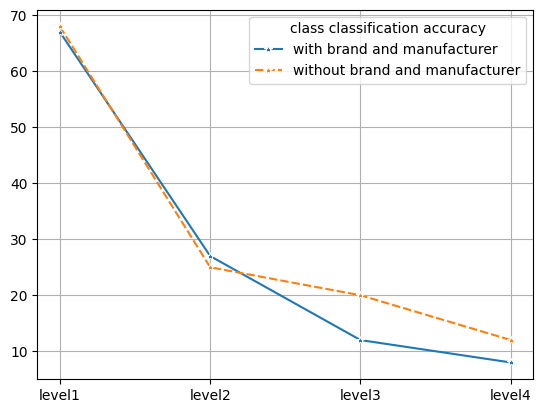
\includegraphics[width=0.8\linewidth]{results_cc_feature}
	\caption{The impact of inlcuding brand and manufacturer in the prompt on class classification accuracy for the 100 randomly selected samples}
	\label{fig:results_cc_feature}
\end{figure}

\subsection{Effect of text generation parameters}\label{hyperparameters-temp}

In investigating the influence of hyperparameters on the generated outputs, our focus was primarily on the temperature parameter, recognized for its pivotal role in balancing creativity and accuracy in language model outputs. Comparing three values—0.5, 0.8, and 1—we maintained consistency in other aspects of the study, particularly the zero-shot approach with category description as the optimal setup. The results showcased that a temperature of 0.8 yielded the best outcomes in terms of class classification metrics (\autoref{fig:results_cc_temp}). While the Flesch reading ease scores among the different temperatures were closely aligned, the average for 0.8 slightly outperformed the others (\autoref{fig:results_flesch_temp}). This underscores the significance of fine-tuning hyperparameters to achieve optimal balance in generating accurate and readable product descriptions.



%\begin{figure}[H]
%	\centering
%	\begin{minipage}{.5\textwidth}
%		\centering
%		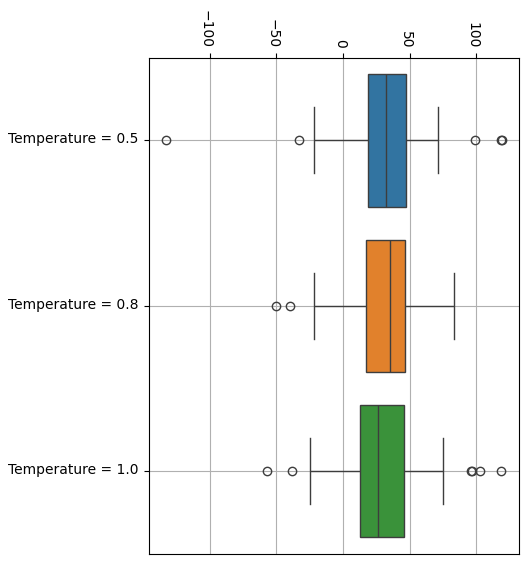
\includegraphics[width=1\linewidth]{results_flesch_temp}
%		\caption{The impact of temperature on Flesch reading ease score for the 100 randomly selected samples}
%		\label{fig:results_flesch_temp}
%	\end{minipage}%
%	\begin{minipage}{.5\textwidth}
%		\centering
%		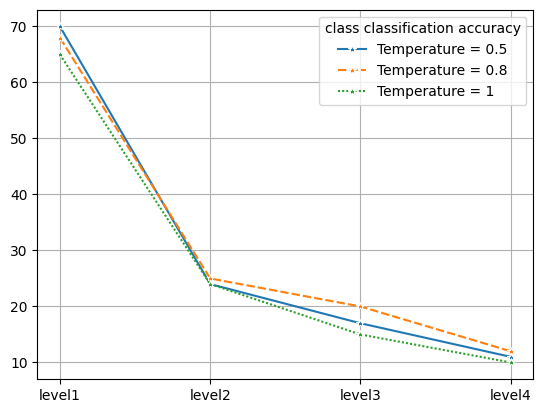
\includegraphics[width=1\linewidth]{results_cc_temp}
%		\caption{The impact of temperature on class classification accuracy for the 100 randomly selected samples}
%		\label{fig:results_cc_temp}
%	\end{minipage}
%\end{figure}

\begin{figure}[H]
	\centering
	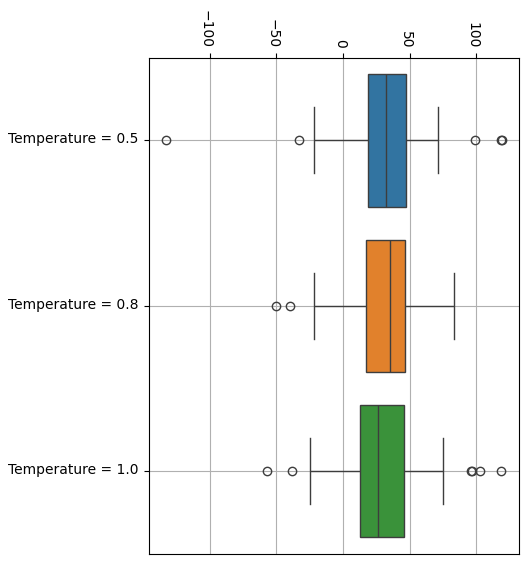
\includegraphics[width=0.5\linewidth]{results_flesch_temp}
	\begin{tabular}{|l|l|l|l|l|}
		\hline
		\textbf{} & \textbf{mean} & \textbf{std} & \textbf{min} & \textbf{max} \\ \hline
		\textbf{Temperature = 0.5} & \textbf{31.19} & \textbf{30.10} & \textbf{-132.58} & \textbf{119.19} \\ \hline
		\textbf{Temperature = 0.8} & \textbf{30.87} & \textbf{25.22} & \textbf{-50.39} & \textbf{82.93} \\ \hline
		\textbf{Temperature = 1.0 } & 28.03  & 28.97  & -57.11  & 118.17 \\ \hline
	\end{tabular}
	\captionlistentry[table]{The impact of temperature on Flesch reading ease score for the 100 randomly selected samples}
	\captionsetup{labelformat=andtable}
	\caption{The impact of temperature on Flesch reading ease score for the 100 randomly selected samples}
	\label{fig:results_flesch_temp}
\end{figure}

\begin{figure}[H]
	\centering
	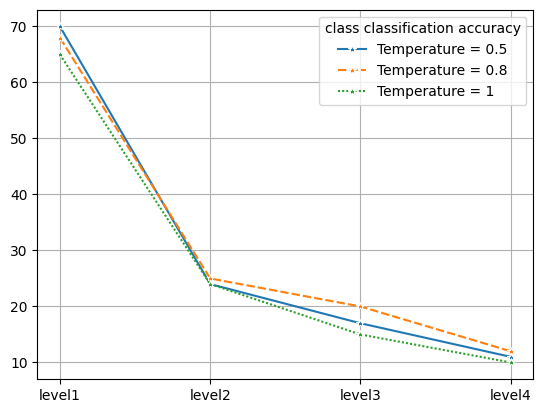
\includegraphics[width=0.8\linewidth]{results_cc_temp}
	\caption{The impact of temperature on class classification accuracy for the 100 randomly selected samples}
	\label{fig:results_cc_temp}
\end{figure}

\subsection{Shots from unrelated vs related category}

In examining the impact of incorporating shots from an unrelated category versus related category into our prompts, we conducted one-shot and two-shot experiments while keeping other study parameters constant. Excluding the categories in our sample group, we selected a random category from the list of categories and generated shots for that category ("Shelf, shelf system (office equipment)"). The results revealed that the one-shot prompt, specifically with related category shots, generated the best output based on the class classification metric. Although the Flesch reading ease scores were closely aligned across different prompt structures, the average for the two-shot prompt with related category shots was slightly higher than the others. Overall, The prompts with related category shots performed better.


%\begin{figure}[H]
%	\centering
%	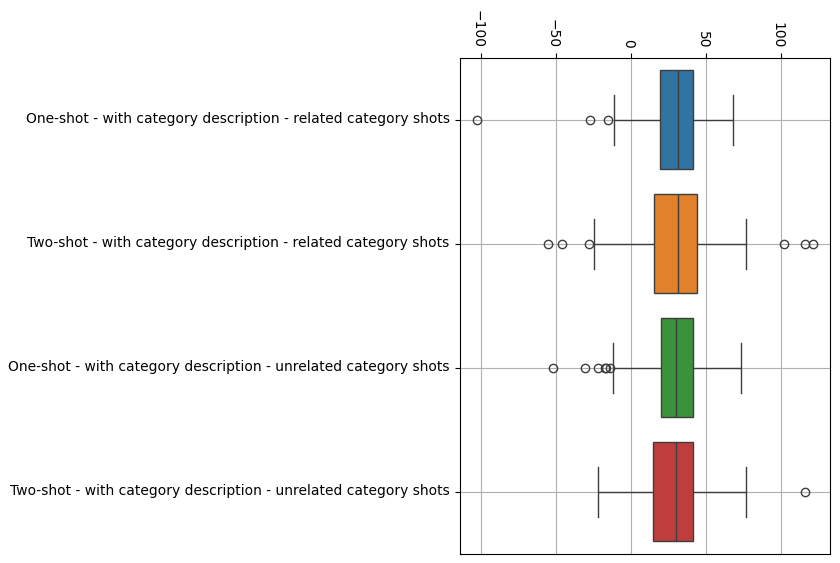
\includegraphics[width=0.5\linewidth]{results_flesch_unrelated}
%	\begin{table}[!ht]
%		\centering
%		
%		\begin{tabular}{|l|l|l|l|l|}
%			\hline
%			\textbf{} & \textbf{mean} & \textbf{std} & \textbf{min} & \textbf{max} \\ \hline
%			\textbf{One-shot - with category description - related category shots} & 28.00 & 22.69 & -102.80 & 68.04 \\ \hline
%			\textbf{Two-shot - with category description - related category shots} & \textbf{30.50} & \textbf{26.67} & \textbf{-55.60} & \textbf{121.22} \\ \hline
%			\textbf{One-shot - with category description - unrelated category shots} & 28.42 & 22.10 & -52.15 & 73.24 \\ \hline
%			\textbf{Two-shot - with category description - unrelated category shots } & 28.77  & 22.02  & -22.40  & 116.14 \\ \hline
%		\end{tabular}
%	\end{table}
%	\captionlistentry[table]{The impact of shots from unrelated vs related Category on Flesch reading ease score for the 100 randomly selected samples}
%	\captionsetup{labelformat=andtable}
%	\caption{The impact of shots from unrelated vs related Category on Flesch reading ease score for the 100 randomly selected samples}
%	\label{fig:results_flesch_unrelated}
%\end{figure}


\begin{figure}[H]
	\centering
	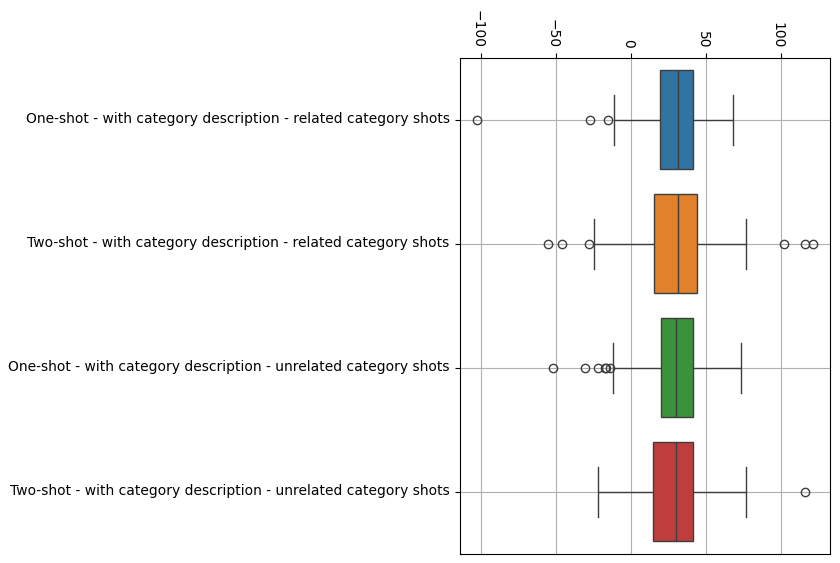
\includegraphics[width=0.5\linewidth]{results_flesch_unrelated}
	\begin{tabular}{|l|l|l|l|l|}
		\hline
		\textbf{} & \textbf{mean} & \textbf{std} & \textbf{min} & \textbf{max} \\ \hline
		\textbf{\makecell{One-shot -\\ with category description -\\ related category shots}} & 28.00 & 22.69 & -102.80 & 68.04 \\ \hline
		\textbf{\makecell{Two-shot -\\ with category description -\\ related category shots}} & \textbf{30.50} & \textbf{26.67} & \textbf{-55.60} & \textbf{121.22} \\ \hline
		\textbf{\makecell{One-shot -\\ with category description -\\ unrelated category shots}} & 28.42 & 22.10 & -52.15 & 73.24 \\ \hline
		\textbf{\makecell{Two-shot -\\ with category description -\\ unrelated category shots} } & 28.77  & 22.02  & -22.40  & 116.14 \\ \hline
	\end{tabular}
	\captionlistentry[table]{The impact of shots from unrelated vs related Category on Flesch reading ease score for the 100 randomly selected samples}
	\captionsetup{labelformat=andtable}
	\caption{The impact of shots from unrelated vs related Category on Flesch reading ease score for the 100 randomly selected samples}
	\label{fig:results_flesch_unrelated}
\end{figure}

\begin{figure}[H]
	\centering
	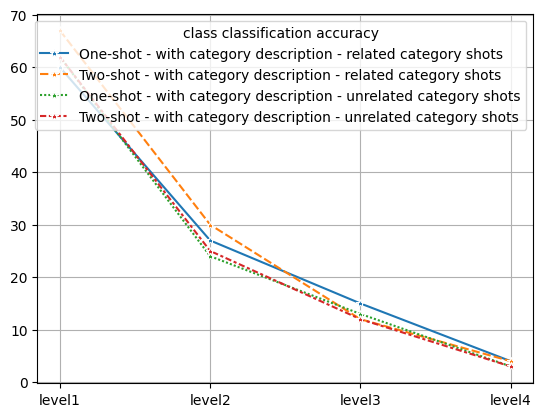
\includegraphics[width=0.8\linewidth]{results_cc_unrelated}
	\caption{The impact of shots from unrelated vs related Category on class classification accuracy for the 100 randomly selected samples}
	\label{fig:results_cc_unrelated}
\end{figure}


\section{Bloom based coherence metric}


In the evaluation of coherence for the optimal scenario (zero-shot with category description), we employed the coherence metric \footnote{The prompt and more details on this metric is avaibale in \autoref{coherence_metric_methods}} on the post-processed text using the German Bloom model. This metric is supposed to provide valuable insights into the logical flow and consistency of the generated product descriptions, contributing additional dimensions to our overall evaluation of the text quality. The results (\autoref{fig:result_coherence}) indicated an average coherence score of 3.46 in the range of 1 to 5, with a maximum score of 4 and a minimum score of 2. 

We chose not to include the coherence metric in our evaluation due to difficulties and uncertainties, which will be discussed fully in the discussion chapter. To briefly summarize, however, the metric's reliance on the same model introduced bias, and issues such as non-numeric character generation and a lack of score variance raised questions about reliability. Inconsistencies between model scoring and human judgment called into question the metric's effectiveness in assessing coherence. Therefore, this metric proved to be unusable and did not provide useful insights, so we decided to refrain from evaluating other prompt settings with this metric. 

%\begin{figure}[H]
%	\centering
%	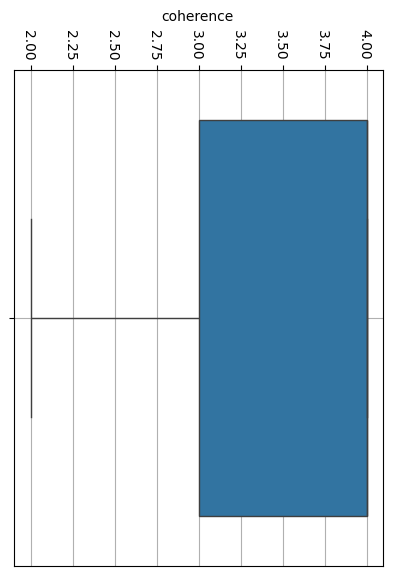
\includegraphics[width=0.8\linewidth]{coherence}
%	\caption{coherence scores of zero-shot with category description for the 100 randomly selected samples}
%	\label{fig:result_coherence}
%\end{figure}

\begin{figure}[H]
	\centering
	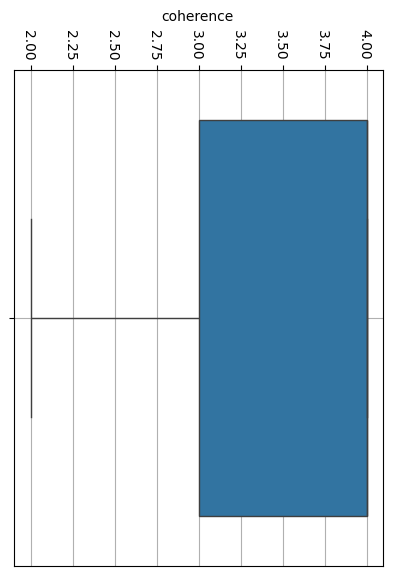
\includegraphics[width=0.5\linewidth]{coherence}
	\begin{tabular}{|l|l|l|l|l|}
		\hline
		\textbf{} & \textbf{mean} & \textbf{std} & \textbf{min} & \textbf{max} \\ \hline
		\textbf{Coherence} & 3.469136  & 0.726058  & 2.000000  & 4.000000 \\ \hline
	\end{tabular}
	\captionlistentry[table]{Coherence scores of zero-shot with category description for the 100 randomly selected samples}
	\captionsetup{labelformat=andtable}
	\caption{Coherence scores of zero-shot with category description for the 100 randomly selected samples}
	\label{fig:result_coherence}
\end{figure}


\section{Study: Q\&A with the bert model}

Regarding class classification with BERT, it's important to note that our study does not prioritize this metric due to the absence of evaluation method for generative outputs and models. We lack a clear accuracy metric for BERT, making it challenging to assess the model's performance objectively. Our exploration of this metric was driven by curiosity rather than a robust evaluation framework. It would also be interesting to compare the performance of this Metric to the PBS class classification model. In this metric, we would ask the Bert model what the product category is based on the product description and then calculate the word vectors for both output of the model and actual category. The output of the model is the cosine similarity of these two vectors. In the optimal scenario of zero-shot with category description, the BERT model yielded an average accuracy of 26\% for the 100 sample products and descriptions. While the lack of a defined accuracy measure limits our ability to thoroughly evaluate BERT's performance, the comparable results to the PBS model suggest that the results obtained from the PBS model and BERT have a degree of correlation.

Given the highly specific category names in the PBS data, the absence of exact matches in the BERT model results led to the use of cosine similarity for evaluating similarity. Further research is needed to establish a calibrated accuracy metric for BERT-based class classification, addressing the current challenge of evaluating the reliability and correctness of the model's performance and assessing relative similarity across all categories in the dataset.

\begin{figure}[H]
	\centering
	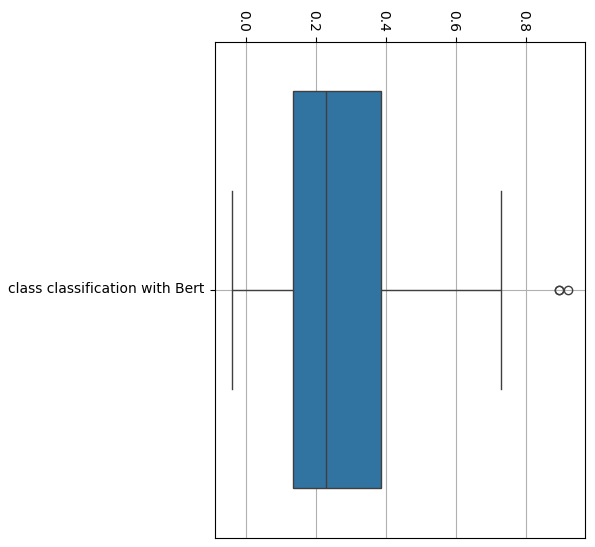
\includegraphics[width=0.7\linewidth]{bert}
	\caption{Class classification scores of outputs for the 100 randomly selected samples using bert model}
	\label{fig:results-bert}
\end{figure}